% Specify the type of document
\documentclass[12pt]{article}

% Load a number of useful packages
\usepackage{graphicx}
\usepackage{amsmath,amssymb,amsfonts,amsthm}
 \usepackage[margin=1.0in]{geometry}
\usepackage[colorlinks=true]{hyperref}
\usepackage{cite}
\usepackage[caption=false,font=footnotesize]{subfig}
\usepackage{float}
\usepackage{float}
\usepackage{enumitem}
\usepackage[export]{adjustbox}
\setlist{nosep,after=\vspace{\baselineskip}}
% Two more packages that make it easy to show MATLAB code
\usepackage[T1]{fontenc}
\usepackage[framed,numbered]{matlab-prettifier}
\lstset{
	style = Matlab-editor,
	basicstyle=\mlttfamily\small,
}

% Say where pictures (if any) will be placed
\graphicspath{{./Pictures/}}

% Define title, author, and date
\title{Drones in Wind}
\author{Nico Alba, Isabel Anderson, Emilio Gordon, Michael Gray, Will Reyes}


% Start of document
\begin{document}

% Put the title, author, and date at top of first page
\maketitle


\section{Goal}
The "Drones in Wind" simulation simulates the flight of a quadcopter drone. The drone in the simulation will be modeled after the AscTec Pelican, a research-drone by the German company Ascending Technologies. The simulated drone as of the point of writing this paper is equipped with sensors to measure the velocity in the horizontal and vertical axis, the vertical position and the pitch angle. The goal is to create a controller that linearizes about a time optimal trajectory given by the third-party program OptimTraj.
%%%%%%%%%%%%%%%%%%%%%%%%%%%%%%%%%%%%%%%%%%%%%%%%%%%%%%%%
%                                                                                 Model                                                                                  %
%%%%%%%%%%%%%%%%%%%%%%%%%%%%%%%%%%%%%%%%%%%%%%%%%%%%%%%%
\section{Model}
The motion of the drone is governed by the ordinary differential equations with the state defined as
\begin{equation}
\label{state}
\dot{x} = \begin{bmatrix} \dot{x}\\ \frac{f\sin{\theta}}{m} \\ \dot{z} \\ \frac{f\cos{\theta}}{m} - g \\ \omega \end{bmatrix}
= \frac{d}{dt}
\begin{bmatrix} x \\ \dot{x} \\ z \\ \dot{z} \\ \theta 
\end{bmatrix}
\end{equation}
such that $x$ and $z$ correspond to horizontal and vertical position, respectively, while $\theta$ corresponds to the angle of the quad from upright. The inputs for the system are defined as
\begin{equation}
\label{inputs}
u = \begin{bmatrix} \omega \\ f \end{bmatrix}
\end{equation}
such that $\omega$ corresponds to angular pitch rate and $f$ corresponds to thrust. Taking the Jacobian lends the following A and B matrices shown by Equation \ref{A_matrix_intermediate} and Equation \ref{B_matrix_intermediate}
\begin{equation}
\label{A_matrix_intermediate}
A = \begin{bmatrix} 0 && 1 && 0 && 0 && 0 \\ 0 && 0 && 0 && 0 && \frac{f\cos{\theta}}{m} \\  0 && 0 && 0 && 1 && 0 \\ 0 && 0 && 0 && 0 && \frac{-f\sin{\theta}}{m} \\ 0 && 0 && 0 && 0 && 0 \end{bmatrix}
\end{equation}

\begin{equation}
\label{B_matrix_intermediate}
B = \begin{bmatrix} 0 && 0 \\ 0 && \frac{\sin{\theta}}{m} \\ 0 && 0 \\ 0 && \frac{\cos{\theta}}{m} \\ 1 && 0 \end{bmatrix}
\end{equation}
There is no need to substitute in equilibrium conditions because we will be linearizing about a trajectory.


%%%%%%%%%%%%%%%%%%%%%%%%%%%%%%%%%%%%%%%%%%%%%%%%%%%%%%%%
%                                                                              Controller                                                                               %
%%%%%%%%%%%%%%%%%%%%%%%%%%%%%%%%%%%%%%%%%%%%%%%%%%%%%%%%
\section{Optimization and Controller}




%%%%%%%%%%%%%%%%%%%%%%%%%%%%%%%%%%%%%%%%%%%%%%%%%%%%%%%%
%                                                                               OptimTraj                                                                             %
%%%%%%%%%%%%%%%%%%%%%%%%%%%%%%%%%%%%%%%%%%%%%%%%%%%%%%%%
\subsection{OptimTraj}

OptimTraj \cite{OptimTraj} was used for trajectory planning. OptimTraj is a MATLAB library designed by a Cornell PHD student, Matthew P. Kelly, to solve for continuous-time single-phase trajectory optimization problems. For OptimTraj to solve the optimal trajectory, you must specify various parameters of your problem, including:
\begin{itemize}
  \item Dynamics
  \item Objective function
  \item Bounds
  \item Initial trajectory guesses
\end{itemize}

The optimal trajectory can now be solved for and subsequently "unpacked". By unpacking the solution, the state and input over time can be tracked and analyzed. One thing to note, however, is that the time-steps of solver matrices do \textbf{not} line up with the simulation time steps provided that run the controller. This is accounted for by modifying the simulation parameters. 
\subsubsection{Function Dynamics}
The simulations begins by setting up the function dynamics, \lstinline!problem.func.dynamics!, as explained in the \textbf{Model} section above: 
\begin{quote}
\begin{lstlisting}
syms xdot x zdot z theta w thrust real
EOMs= [xdot;
       (thrust/mass)*sin(theta);
       zdot;
       (thrust/mass)*cos(theta)-gravity;
       w];

numf = matlabFunction(EOMs,'vars',[x xdot z zdot theta w thrust]);
problem.func.dynamics= @(t,x,u) numf( x(1,:),x(2,:),x(3,:),x(4,:),x(5,:),
                                      u(1,:),u(2,:)) );

\end{lstlisting}
\end{quote}

\subsubsection{Problem Bounds}
The next step is to set up the \lstinline!problem.bounds!. For the function dynamics, a mass-normalized thrust was chosen to keep the model simple, shown in table \ref{Problem Bounds} below. These parameters were chosen so that results of the simulation can be compared to results from D'Andrea's paper\cite{D'Andrea}. 

\begin{table}[H]
\begin{center}
\begin{tabular}{ |p{2.5cm}||p{2cm}||p{3cm}| }

 \hline
 Parameter & Value & Description\\
 \hline
 $t_{i}$   & 0 s  & Initial time\\
 $t_{f}$  & 2 s  & Final time\\
 $\underline{F}/m$ & 1 m/$s^{2}$ & Min thrust\\
 $\overline{F}/m$ & 20 m/$s^{2}$ & Max thrust\\
 $\overline{\omega}$ & 10 rad/s & Max pitch rate \\
 \hline
\end{tabular}
\caption{Problem Bounds }
\label{Problem Bounds}
\end{center}
\end{table}



\subsubsection{Cost Function}
Using a cost function, an optimized trajectory around any aspect of the simulation can be found. The cost functions available for different variables are shown below. 
\begin{quote}
\begin{lstlisting}
% Input:
problem.func.pathObj = @(t,x,u)( sum(u.^2,1) );

% Thrust:
problem.func.pathObj = @(t,x,u)( sum(u(2,:).^2,1) );

% Pitch Rate:
problem.func.pathObj = @(t,x,u)( sum(u(1,:).^2,1) );

% Time
problem.func.pathObj = @(t,x,u)( sum((x(1,:)-x_f).^2,1) 
                                +sum((x(3,:)-z_f).^2,1))

% Time objective function for boundary points
problem.func.bndObj = @(t0,x0,tF,xF) (tF-t0)

\end{lstlisting}
\end{quote}
For our purposes, we explicitly used the "Time objective function for boundary points" and the other cost functions were commented out.

\clearpage

\subsubsection{Initialize Guess}
Lastly, before running the solution, the solver must be initialized. This is done with the mandatory \lstinline!problem.guess! struct. Where $x_{i}$ and $x_{f}$ are the desired initial and final states, respectively. Additionally, $u_{i}$ and $u_{f}$ are the desired initial and final input, respectively. 

\begin{figure}[H]
\begin{equation*}
\lstinline!problem.guess.time! = [t_{i}, t_{f}]
\end{equation*}
\begin{equation*}
\lstinline!problem.guess.state! = [x_{i}, x_{f}]
\end{equation*}
\begin{equation*}
\lstinline!problem.guess.control! = [u_{i}, u_{f}] 
\end{equation*}
\end{figure}
\subsubsection{Options}
Additional options are available using \lstinline!problem.options!, which include details to change accuracy settings and select different solution methods, like trapezoid, Chebyshev, etc.
\subsubsection{Solution}
Finally, running the command \lstinline!soln = optimTraj(problem)! is used to solve. Following this, it is possible to unpack the simulation, save the data, and plot it.
\begin{quote}
\begin{lstlisting}
t = linspace(soln.grid.time(1),soln.grid.time(end),soln.grid.time(end)*TimeDensity);
x = soln.interp.state(t);
u = soln.interp.control(t);
save('traj.mat','t','x','u');
\end{lstlisting}
\end{quote}

The reason the time grid-spacing is the end-time multiplied by \lstinline!TimeDesnity! is to keep the grid-spacing of the simulation and optimal trajectory path the same. This will be elaborated on further in Section \ref{Running Simulation}.

%%%%%%%%%%%%%%%%%%%%%%%%%%%%%%%%%%%%%%%%%%%%%%%%%%%%%%%%
%                                                                               Controller                                                                              %
%%%%%%%%%%%%%%%%%%%%%%%%%%%%%%%%%%%%%%%%%%%%%%%%%%%%%%%%
\subsection{Controller}
The controller is designed to use in the loop control with LQR to follow a given trajectory. First, the init function creates a symbolic description of the A and B matrices, in which the angle $\theta$ and the thrust $f$ are the only variables.  These symbolic descriptions are then turned into MATLAB functions and saved in the data struct.  The Q and R weight matrices are then initialized.  The init function proceeds to load in the trajectory data and also adds it to the data struct.  Finally, some parameters used to determine when the quad has reached its destination are initialized.
\begin{quote}
\begin{lstlisting}
% Create functions
data.funcA = matlabFunction(A);
data.funcB = matlabFunction(B);

% Trajectory
load('traj.mat')
\end{lstlisting}
\end{quote}

Logic is used at the start of the control loop to determine if there is still trajectory data available for the current timestep.  If there is not, the controller will linearize about the last available trajectory point.
\begin{quote}
\begin{lstlisting}
% Reference trajectory
ind = data.index;
if data.index < length(data.trajT)
    trajX = data.trajX(ind);
    trajXdot = data.trajXdot(ind);
    trajZ = data.trajZ(ind);
    trajZdot = data.trajZdot(ind);
    trajTheta = data.trajTheta(ind);
    trajW = data.trajW(ind);
    trajF = data.trajF(ind);
    data.index = data.index + 1;


\end{lstlisting}
\end{quote}
Where \lstinline!data.index! is initialized at 1. 
\newline
\newline
After determining that the simulation is still within the regime in which a trajectory is available, the controller will find the respective trajectory point to linearize about for the current time-step.  The angle and thrust for this trajectory point is passed into the MATLAB functions to determine the relevant A and B matrices, which are then used in conjunction with the already initialized weights to create a gain matrix using LQR.
\begin{quote}
\begin{lstlisting}
A = data.funcA(trajTheta,trajF);
B = data.funcB(trajTheta);
data.K = lqr(A,B,data.Q,data.R);

\end{lstlisting}
\end{quote}

Finally, the input $u = -Kx + n$ is applied in which $K$ is the previously specified gain matrix, $x$ is the difference between the current state and the trajectory state at the current time, and $n$ is the trajectory input at the current time. As an example, when the quadroter is meant to be at hover, $n = -mg$.

\clearpage
%%%%%%%%%%%%%%%%%%%%%%%%%%%%%%%%%%%%%%%%%%%%%%%%%%%%%%%%
%                                                                         Running Simulation                                                                                %
%%%%%%%%%%%%%%%%%%%%%%%%%%%%%%%%%%%%%%%%%%%%%%%%%%%%%%%%
\section{Running Simulation}\label{Running Simulation}

To run the simulation, a function named \lstinline!automation.m! was used to set up the problem bounds, plan the optimal trajectory, and analyze the results. Shown below is the script to do so.
\begin{quote}
\begin{lstlisting}
% Constants to be applied
clear; 

TimeDensity = 400;
xFinal = 5;
zFinal = 5;
runTime = 2;

gravity = 9.81;
mass = 1;

maxPitchRate = 10;
maxThrust = 20;
minThrust = 1;

save('runOptions.mat');

%Run the three scripts
planOptimalTrajectory()
DesignProblemSummer2017('Controller','datafile','data.mat')
AnalysisOfOptimalTrajectory()

\end{lstlisting}
\end{quote}
\lstinline!TimeDensity! refers to the grid-spacing in the optimal trajectory solution as well as the time-step for \lstinline!DesignProblemSummer2017!. The other options set problem bounds and save them into \lstinline!runOptions.mat! to be used by the DesignProblem, controller, and the Optimal trajectory planner. 
\newline
\newline
\lstinline!AnalysisOfOptimalTrajectory()! plots the simulation against the optimal trajectory calculated by optimTraj.
%%%%%%%%%%%%%%%%%%%%%%%%%%%%%%%%%%%%%%%%%%%%%%%%%%%%%%%%
%                                                                                Analysis  of Optimal Trajectory  %
%%%%%%%%%%%%%%%%%%%%%%%%%%%%%%%%%%%%%%%%%%%%%%%%%%%%%%%%
\section{Analysis of Optimal Trajectory}

In this section, the trajectory for $x=5,z=5$ was analyzed. First the Optimal trajectory was calculated and saved, then the simulation was run and data stored, and finally both results were plotted against each other. \textbf{Solid lines} show the optimal trajectory, and \textbf{dashed lines} show the simulated quad-rotor path.

Ultimately, the results will be compared to \textbf{one} of D'Andrea's results\cite{D'Andrea}. 

%%%%%%%%%%%%%%%%%%%%%%%%%%%%%%%%%%%%%%%%%%%%%%%%%%%%%%%%
%                                                                                Simulation Analysis               %
%%%%%%%%%%%%%%%%%%%%%%%%%%%%%%%%%%%%%%%%%%%%%%%%%%%%%%%%
\clearpage
\subsection{Simulation Analysis}

\begin{quote}
\begin{lstlisting}
load traj
topt = t;
xopt = x;
uopt = u;

load data
tsim = processdata.t;
xsim = [processdata.x; processdata.xdot; processdata.z; processdata.zdot;    processdata.theta];
usim = [controllerdata.actuators.pitchrate;...
	controllerdata.actuators.thrust];
\end{lstlisting}
\end{quote}
The preceding lines of code are meant to show how easily the data can be unpacked and plotted against each other. Below, Figure \ref{State Plot} shows the optimal and actual state of the quadrotor, and Figure \ref{Input Plot} shows the optimal and actual inputs of the quadrotor.
\newline
\newline







%%%%%%%%%%%%%%%%%%%%%%%%%%%%%%%%%%%%%%%%%%%%%%%%%%%%%%%%
%                                                          Comparison with D'Andrea Results                %
%%%%%%%%%%%%%%%%%%%%%%%%%%%%%%%%%%%%%%%%%%%%%%%%%%%%%%%%
\subsection{Comparison with D'Andrea Results}

We can compare the simulated trajectory with that of \textit{Performance Benchmarking of Quadrotor Systems Using Time-Optimal Control} \cite{D'Andrea}. The trajectory to be compared to from D'Andrea's paper is shown in Figure \ref{D'Andrea Plot}

Reminder, \textbf{Solid lines} show the calculated optimal trajectory. \textbf{Dashed lines} show the simulated quad-rotor path.

\begin{figure}[h!]
  \centering
  \begin{minipage}[b]{0.49\textwidth}
    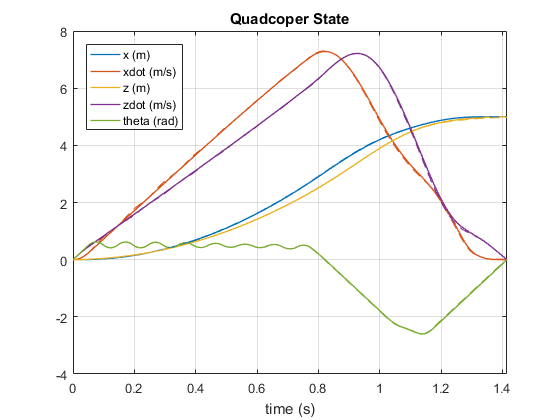
\includegraphics[width=\textwidth]{State.png}
    \caption{\label{State Plot} Quadcopter state over time.}
  \end{minipage}
  \hfill
  \begin{minipage}[b]{0.49\textwidth}
    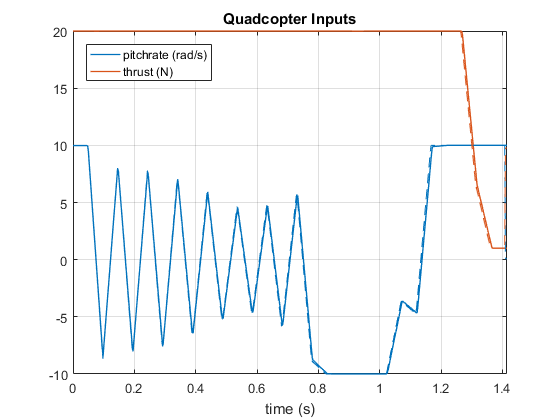
\includegraphics[width=\textwidth]{Inputs.png}
    \caption{\label{Input Plot} Quadcopter Inputs over time.}
  \end{minipage}
\end{figure}

\begin{figure}[H]
\centerline{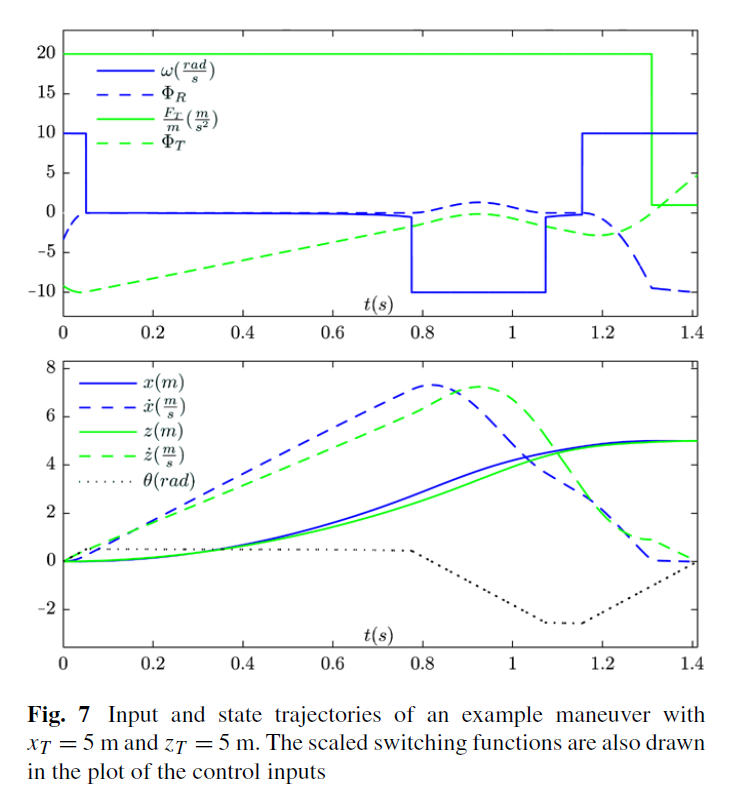
\includegraphics[width=9cm, height=8.5cm]{DAndrea_55_Plot.png}}
  \caption{\label{D'Andrea Plot} Screenshot of D'Andrea Results}
  \label{fig}
\end{figure}

Though both results are nearly identical, the biggest difference in performance is in that of the inputs. 
D'Andrea input for thrust is bang-bang, meaning there is a switch discontinuity and the input only takes the minimum and maximum values \cite{BangBangControl}. D'Andrea's pitch rate is bang-singular, meaning the control input is always at full positive or negative saturation, except during singular arcs \cite{D'Andrea}.

In our model, the inputs were free to vary as continuously as possible between the bounds set in table \ref{Problem Bounds}. Despite this, both models arrived at the destination $x=z=5$ following approximately the same time-optimal path and input behavior. In order to completely match input behavior, this issue may be resolved through tinkering with OptimTraj.


%%%%%%%%%%%%%%%%%%%%%%%%%%%%%%%%%%%%%%%%%%%%%%%%%%%%%%%%
%                                                                              D'Andrea Results                                                                        %
%%%%%%%%%%%%%%%%%%%%%%%%%%%%%%%%%%%%%%%%%%%%%%%%%%%%%%%%



%%%%%%%%%%%%%%%%%%%%%%%%%%%%%%%%%%%%%%%%%%%%%%%%%%%%%%%%
%                                                                                Future Work                                                                         %
%%%%%%%%%%%%%%%%%%%%%%%%%%%%%%%%%%%%%%%%%%%%%%%%%%%%%%%%
\section{Future Work}
With the completion of a 2D optimized drone path, plans to enhance the simulation are underway. Two main additions will be added to the current simulation in order to complete this task. Those are as follows 
\newline
\begin{itemize}
  \item Implement 3D rigid body dynamics
  \item Implement additional aerodynamic forces such as drag and ground effect
\end{itemize}
\textit{Controlling of an Single Drone}\cite{Controlling of an Single Drone} provides an outline for how to linearize a 3D quadcopter using rigid body dynamics. A key difference to note is that in the dynamics discussed in \cite{Controlling of an Single Drone}, each of the four quadrotor blades can produce its own thrust, which will then control the pitch, roll, and yaw of the rigid body. Additionally, the paper gives a brief description of the mechanism on applying aerodynamic forces, namely, drag.


% Display list of references in IEEE Transactions format.
\clearpage
% Display list of references in IEEE format.



\begin{thebibliography}{9}


\bibitem{Controlling of an Single Drone}
Emile Biever
\textit{Controlling of an Single Drone}.
TU/E Eindhoven: Department of Mechanical Engineering, 2015.



\bibitem{OptimTraj} 
Matthew Peter Kelly
\textit{OptimTraj}
GitHub
\\\texttt{https://github.com/MatthewPeterKelly/OptimTraj}


\bibitem{BangBangControl}
Nguyen Tan Tien
\textit{Introduction to Control Theory Including Optimal Control}.
C.11 Bang-bang Control:53-58, 2002
\\\texttt{https://goo.gl/pj9oyA}
% Too long to fit:
%  http://www4.hcmut.edu.vn/~nttien/Lectures/Optimal%20Control/C.11%20Bang-bang%20Control.pdf



\bibitem{D'Andrea}
Rafaello D'Andrea
\textit{Performance Benchmarking of Quadrotor Systems Using Time-Optimal Control}.
Auton Robot, 33:69-88, 2012.















\end{thebibliography}


% End of document (everything after this is ignored)
\end{document}